\documentclass[11pt]{article}
\usepackage[utf8]{inputenc}
\usepackage[T1]{fontenc}
\usepackage{lmodern}
\usepackage{amsmath,amssymb}
\usepackage{graphicx}
\usepackage{booktabs}
\usepackage[margin=2.5cm]{geometry}
\usepackage{xcolor}
\usepackage[numbers,sort&compress]{natbib}
\usepackage{hyperref}
\newcommand{\tocomplete}[1]{\textcolor{red}{[To be completed: #1]}}

\title{Service failures of learned multi-agent signal controllers on a two-intersection corridor:\\
an evaluation with optimised fixed plans and paired protection ablations}
\author{\tocomplete{authors and affiliations}}
\date{Draft of \today{} --- development results; not peer reviewed}

\begin{document}
\maketitle

\begin{abstract}
We study three value-based multi-agent reinforcement learning controllers (QMIX, VDN and independent DQN)
on a SUMO corridor of two signalised intersections spaced 300\,m apart, with decisions every 5\,s between
extending the current green and switching through a 3\,s yellow. The evaluation keeps every run, including
runs that fail to clear the network, and compares the learned policies with fixed plans optimised on
separate traffic samples, one of them re-optimised under the same 7\,s minimum green. On five development
traffics, the historical fixed plan obtains a lower mean waiting burden than every learned method, and the
re-optimised constrained plan remains competitive with the historical QMIX policies. Inspecting the
failures shows a mechanism that mean metrics hide: after the demand ends, a greedy policy can enter a
nearly stationary state in which an isolated vehicle on a red approach is never served. We then add two
protections at inference time, to policies trained without them --- a 7\,s minimum green and a service guarantee whose counter is provably
bounded by 127\,s --- and measure their effects on the same models and traffics (600 paired evaluations).
The guarantee cleared all six failed runs, intervening once per run and only after the demand had ended,
so its cost during the demand was not exercised; the minimum green raised the waiting burden of every QMIX
and VDN policy (by 1.2--2.3\,s per vehicle) and had mixed effects on IDQN. The comparison under this common
constraint is asymmetric: the fixed plan was re-optimised for it, whereas the historical policies were trained
without it and constrained only at evaluation, without retraining; none of their 299 runs that cleared matched
that plan (the 300th failed to clear). Single-seed pilots trained with both protections give an exploratory,
unfavourable signal; they do not indicate how a full multi-seed training campaign would turn out. The results
are development evidence on already-inspected traffics; a robustness study on new traffics is prepared, and a
decision on retraining is deferred.
\end{abstract}

\section{Introduction}
Deep reinforcement learning (RL) controllers for traffic signals are commonly reported to reduce delays
relative to fixed-time or actuated control \cite{wei2018intellilight,wei2019presslight,wei2019colight,chen2020thousand,chu2020multiagent,haydari2022survey,noaeen2022review}.
Two features of how these comparisons are usually made limit what they show. First, the reference plans are
often not optimised under the same operational constraints as the learned controller, which has been
pointed out for fixed-time baselines in particular \cite{ault2020interpretable,ault2021resco}. Second, the
headline metrics are averages over completed trips or over successful episodes; a controller that
occasionally leaves a vehicle waiting indefinitely can look good on such averages, and evaluation practice
in deep RL more broadly is sensitive to such reporting choices \cite{henderson2018matters,agarwal2021precipice,jayawardana2022underspecification,varela2021methodology}.

We examine these two issues on a deliberately small and fully controlled case: two intersections, three
value-based multi-agent methods with centralised (QMIX \cite{rashid2020qmix}, VDN \cite{sunehag2018vdn}) or
independent (IDQN \cite{tampuu2017multiagent,mnih2015human}) training, and fixed plans searched on separate
traffic samples. The questions are:
\begin{enumerate}
\item On the same traffics, how do the learned controllers compare with optimised fixed plans, including a
plan optimised under the same minimum green?
\item When a learned controller fails to clear the network, what happens, and is it visible in the usual
metrics?
\item What do two simple protections --- a minimum green and a service guarantee --- change when added at
evaluation time to policies trained without them, on efficiency and on service?
\end{enumerate}
The contribution is empirical and methodological. Minimum greens and action masks are standard
\cite{huang2022masking,alshiekh2018shielding}; we do not claim novelty for them. What we report is (i) a
hash-verified comparison with constrained optimised fixed plans, (ii) a documented failure mechanism of
greedy learned policies after the demand ends, and (iii) a paired measurement, on identical models and
traffics, of what each protection costs during the demand and what it changes afterwards.

\section{Related work}
\paragraph{Learned signal control.}
Single-agent and multi-agent deep RL controllers include IntelliLight \cite{wei2018intellilight},
PressLight \cite{wei2019presslight}, CoLight \cite{wei2019colight}, FRAP \cite{zheng2019frap},
MPLight \cite{chen2020thousand} and multi-agent actor--critic methods \cite{chu2020multiagent}; earlier
multi-agent work includes MARLIN-ATSC \cite{eltantawy2013marlin}. Surveys \cite{haydari2022survey,noaeen2022review}
and benchmark libraries \cite{ault2021resco,mei2024libsignal,bokade2025pytsc} document the field. PyTSC
\cite{bokade2025pytsc} compares IQL, VDN and QMIX on SUMO grids; in generic cooperative tasks, independent
learning is often competitive with value factorisation \cite{papoudakis2021benchmarking}.
\tocomplete{confirm the network, constraint and baseline details of these works from the full texts (only
abstracts and metadata were checked for this draft)}.

\paragraph{Model-based adaptive control and service.}
Max pressure has throughput guarantees \cite{varaiya2013max}; its cyclical variant prevents a phase from
being skipped indefinitely \cite{levin2020cyclical}. Queue-based pressure control can leave a lightly loaded
movement waiting, which motivated delay-based back-pressure with fairness properties \cite{wu2018delay}.
Fairness has also been added to the RL objective \cite{raeis2021fair}.

\paragraph{Constraints on learned actions.}
Masking invalid actions and shielding a learner with an external monitor are established
\cite{huang2022masking,alshiekh2018shielding}. Our masks are simple instances of this idea; their interest
here lies in the paired measurement, not in the mechanism.

\section{Environment and controllers}
\paragraph{Network and demand.}
The SUMO \cite{lopez2018sumo} network has two signalised intersections (J1, J2) on a two-lane main axis;
the central link is 279.2\,m long (300\,m between intersections). Each intersection has two phases, main (H)
and secondary (V). Demand is generated over one hour by a conditioned multinomial model with fixed counts:
900 (west$\to$east) and 700 (east$\to$west) main-axis vehicles and 300 per secondary stream (four streams),
2{,}800 vehicles in total. Simulation continues until the network clears or until 7{,}200\,s.

\paragraph{Learned controllers.}
Each agent observes eight normalised local features (halting queues on H and V, current phase, elapsed
green, recent arrival rates on H and V, downstream occupancies). Actions are EXTEND (5\,s more green) and
SWITCH (3\,s yellow then 2\,s of the other green), decided synchronously every 5\,s. The shared reward is
the negative number of stopped vehicle-seconds plus due-but-not-inserted vehicle-seconds over the 5\,s
block. Each agent uses a multilayer perceptron (8--128--128--2); QMIX adds a monotonic mixer conditioned on
the joint 16-dimensional observation (mixing width 32, hypernetwork width 64) \cite{rashid2020qmix}; VDN sums
the agent values \cite{sunehag2018vdn}; IDQN trains each agent independently. All use double-Q targets
\cite{vanhasselt2016double}, a 200{,}000-transition replay, batch 256, learning rate $5\cdot10^{-4}$,
$\gamma=0.99$ per 5\,s, $\varepsilon$ decaying from 1 to 0.05 over 250{,}000 transitions, and
360{,}000 transitions per training. Ten training seeds per method were run; one checkpoint per training was
selected by a fixed rule on separate validation traffics (eligibility on hard validity gates, then minimum
mean waiting burden, then minimum time loss, then earliest checkpoint).

\paragraph{Fixed plans.}
Two-phase fixed plans with common cycle, green split and offset were searched on separate design traffics and
selected on separate validation traffics. The historical plan has a 19\,s cycle with 8\,s and 5\,s greens and
a 9\,s offset. Because a 5\,s green violates the 7\,s minimum adopted below, the search was repeated with
greens of at least 7\,s, giving a 25\,s cycle with 12\,s and 7\,s greens and zero offset (selection on the same
design and validation samples as the original search, so this selection is not an independent validation).

\paragraph{Protections.}
\emph{Minimum green} $G=7$\,s forbids SWITCH while the current green has lasted less than $G$; with the
5\,s clock and the 3+2\,s switch, realised greens are $2+5k$\,s, and 7\,s is the smallest realisable value
above 5\,s. \emph{Service guarantee}: for each red direction a counter increases every second while at least
one vehicle halts on its observed incoming lanes, and resets on green or when the queue empties; when it
reaches $T=120$\,s, EXTEND is forbidden. Both are applied as a mask outside the agents: the executed action
is the greedy action if allowed, otherwise the other action. Under the 5\,s/3+2\,s executor the two masks
never forbid both actions when $T\ge G$, and the counter never exceeds $T+4+3=127$\,s. The bound concerns
the counter (continuous presence of a queue on a red approach), not the cumulative waiting time of a vehicle
or its arrival.

\section{Experimental method}
\paragraph{Traffics.} All results below use five development traffics (seeds 9301--9305), each with its own
SUMO seed. They had been inspected before this study; the results are therefore development evidence and not
a final test.

\paragraph{Indicators.}
$J$ is the mean over the 2{,}800 scheduled vehicles of SUMO waiting time plus departure delay, defined only
when the network clears; failed runs are kept and counted, never imputed. Because $J$ is undefined for a
failure, we also report the waiting burden \emph{during the demand},
\[ D=\sum_{t=1}^{3600}\big(n_{\mathrm{stopped}}(t)+n_{\mathrm{pending}}(t)\big)\ \text{vehicle-seconds},\qquad \bar D = D/N, \]
with $N=2{,}800$, which is defined for every run. Service is described separately by (a) the service
counter, (b) the access time to the first green of a waiting direction, (c) stop-line crossings (main axis
only), and (d) arrivals (per-vehicle waiting time and time loss).

\paragraph{Ablation design.}
The 30 selected checkpoints (3 methods $\times$ 10 seeds) are evaluated greedily on the five traffics under
four arms: no protection, guarantee only, minimum green only, both. This gives 600 evaluations in
$150$ blocks of four paired runs. Fifty QMIX runs without protection were taken from an earlier evaluation
with the same checkpoints, traffics and simulator seeds; their files were hash-verified unchanged. An earlier
technical check, whose log is not part of the present data package, found that the evaluator used for the new
runs reproduces the frozen output files byte for byte in the absence of protection.
\tocomplete{attach the log of that check to the replication package} Effects are paired differences within blocks; $\Delta J$
uses only blocks where both runs clear, and their number is reported. The analysis is descriptive: models and
traffics are crossed factors and no pooled hypothesis test is made.

\section{Results}
\subsection{Learned controllers and fixed plans on the same traffics}
Table~\ref{tab:same} and Figure~\ref{fig:same} report every evaluation on the five traffics. The historical
fixed plan has the lowest mean $J$ (2.772\,s). Re-optimising the fixed plan under the 7\,s minimum green
raises its $J$ to 3.156\,s while lowering its mean time loss from 11.74 to 10.13\,s, an example of the two
indicators disagreeing. The ten historical QMIX policies obtain 3.106\,s on 49 valid runs out of 50; VDN
3.133\,s (50/50) and IDQN 6.123\,s (46/50). No learned run that cleared has a lower $J$ than the historical fixed plan on the same traffic
(145 of the 150 unprotected runs cleared; over the four arms of Section~\ref{sec:protections}, 594 of 600). Without the minimum green, QMIX and VDN obtain a lower $J$ than the constrained plan in 33
of 49 and 30 of 50 runs, but they do so with 2\,s greens (57--61\,\% of their greens during the demand) that
the constrained plan is not allowed; their mean time loss is never lower than that plan's. Single-seed pilots
trained with both protections obtained mean values of 4.32--5.48\,s, above both fixed plans. This is an
exploratory, unfavourable signal only: one training seed per method, no pairing by seed with the ten
historical policies, and no indication of how a full multi-seed campaign would turn out.

\begin{table}[t]
\centering
\caption{Development traffics 9301--9305. $J$ is averaged over cleared runs only; $n$ is the number of
cleared runs. Time loss is the mean over completed vehicles of each run, averaged over the cleared runs. Pilot rows: one training seed each, trained
with both protections, two checkpoints.}
\label{tab:same}
\begin{tabular}{lrrr}
\toprule
Controller & cleared / runs & mean $J$ (s) & mean time loss (s)\\
\midrule
Historical fixed plan (C 19\,s, 8/5\,s, offset 9\,s) & 5/5 & 2.772 & 11.74\\
Fixed plan, greens $\ge$ 7\,s (C 25\,s, 12/7\,s) & 5/5 & 3.156 & 10.13\\
QMIX, 10 policies, no protection & 49/50 & 3.106 & 12.15\\
VDN, 10 policies, no protection & 50/50 & 3.133 & 12.08\\
IDQN, 10 policies, no protection & 46/50 & 6.123 & 19.54\\
QMIX pilot, 250k / 360k transitions & 5/5, 5/5 & 4.698 / 4.435 & 14.02 / 13.57\\
VDN pilot, 250k / 360k & 5/5, 5/5 & 4.324 / 4.815 & 13.23 / 14.59\\
IDQN pilot, 250k / 360k & 5/5, 5/5 & 5.478 / 4.898 & 14.95 / 13.91\\
\bottomrule
\end{tabular}
\end{table}

\begin{figure}[t]
\centering
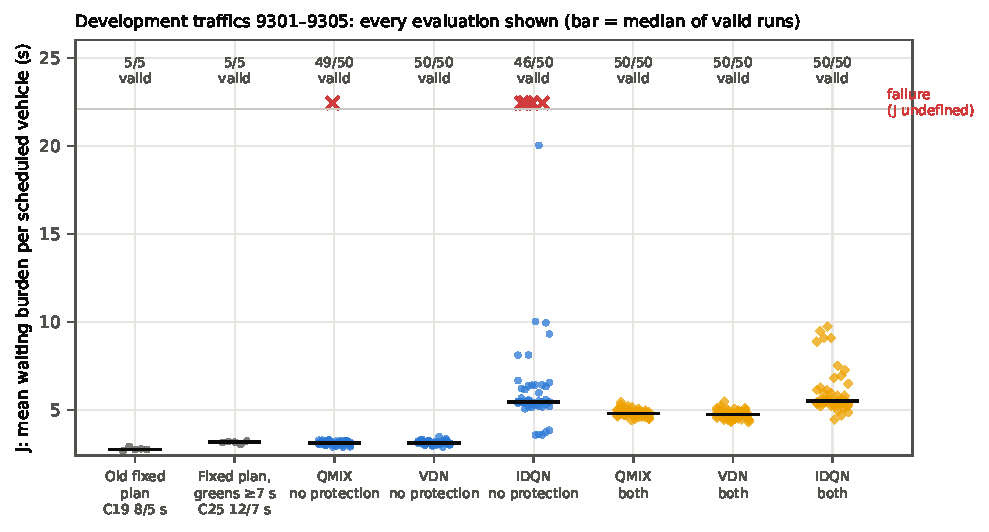
\includegraphics[width=\linewidth]{../figures/fig1_same_traffic_performance}
\caption{Every evaluation on the five development traffics. Failed runs are drawn as crosses in a separate
band and are not averaged; counts above each group.}
\label{fig:same}
\end{figure}

\subsection{Anatomy of a clearance failure}
The QMIX failure (one policy, one traffic) leaves a single vehicle: the last vehicle of a secondary stream,
inserted at 3{,}578\,s, halted at the stop line from 3{,}605\,s to the 7{,}200\,s cut-off, with no other
vehicle in the network after 3{,}679\,s and no insertion backlog. A 2\,s secondary green ended just before the
vehicle reached the stop line; afterwards the intersection's observation became nearly stationary (one halted
vehicle on the secondary approach, no arrivals, main green), and only the elapsed-green feature changed.
Along the logged trajectory the greedy margin $Q(\text{EXTEND})-Q(\text{SWITCH})$ grew from 0.24 to 0.62 as
that feature saturated, so the policy extended the main green at all 718 remaining decisions. The same policy
cleared another traffic only after a 338\,s wait at the other intersection, where the same feature drifted
the margin across zero. Every failure in this study (one QMIX and four IDQN runs without protection, one
IDQN run under the minimum green alone) concerns the last one or two vehicles of a secondary stream, left after
the demand: one unfinished vehicle in five runs, two in one run.
The executed phases were logged as commanded by the controller; a read-back of SUMO's signal state is
available only for the new evaluations, where it showed no mismatch.

\subsection{Effects of the protections}\label{sec:protections}
\paragraph{Guarantee.} With the guarantee alone, all 150 runs cleared (QMIX 50/50, VDN 50/50, IDQN 50/50,
against 49, 50 and 46 without protection). It intervened once in each of 13 runs, always after 3{,}600\,s;
it never intervened during the demand. Consequently the waiting burden during the demand was identical to the
unprotected run in all 150 pairs ($\Delta D=0$), and $\Delta J$ was zero except in pairs where a late
intervention shortened a wait (at most $-0.075$\,s). The maximum counter was 127\,s, as the bound requires,
but the largest cumulative waiting time of a vehicle reached 169\,s: a vehicle can wait at both intersections,
and the counter resets when a queue empties, so the bound does not apply to vehicle waits.

\paragraph{Minimum green.} For QMIX and VDN the effect was regular and large: $\Delta D>0$ in 100/100 pairs,
$\Delta J$ between $+1.29$ and $+2.28$\,s (QMIX, 49 comparable pairs) and between $+1.20$ and $+2.30$\,s (VDN,
50 pairs), and higher time loss in every pair. The mask overrode about 350 decisions per run (QMIX median).
For IDQN the effect was variable: $\Delta D$ was positive in 25 and negative in 25 of 50 pairs (median
$+56$\,veh\,s, range $-35{,}004$ to $+4{,}514$), the median $\Delta J$ was $-0.06$\,s over 45 comparable
pairs, and the minimum green cleared four failed runs but created one.

\paragraph{Both protections.} The combination cleared 150/150 runs. Because the guarantee never acted during
the demand, the interaction contrast on $D$ was zero in all 150 blocks, and on $J$ it was zero or below
0.14\,s in absolute value.

\paragraph{Re-optimised fixed plan versus historical policies constrained at evaluation.} The two sides of
this comparison were not treated alike: the fixed plan was re-optimised for the 7\,s minimum green, whereas the
learned policies are the historical ones, trained without it and constrained only at evaluation, without
retraining. Under the 7\,s minimum green (arms with the minimum green), 299 of these 300 runs cleared, and none of these 299 had a lower $J$ or a lower mean time loss
than the constrained fixed plan on the same traffic (mean differences $+1.58$ to $+2.82$\,s in $J$ by method).
The remaining run (IDQN, minimum green only) failed to clear; it has no $J$ and is not counted as a comparison.

\begin{figure}[t]
\centering
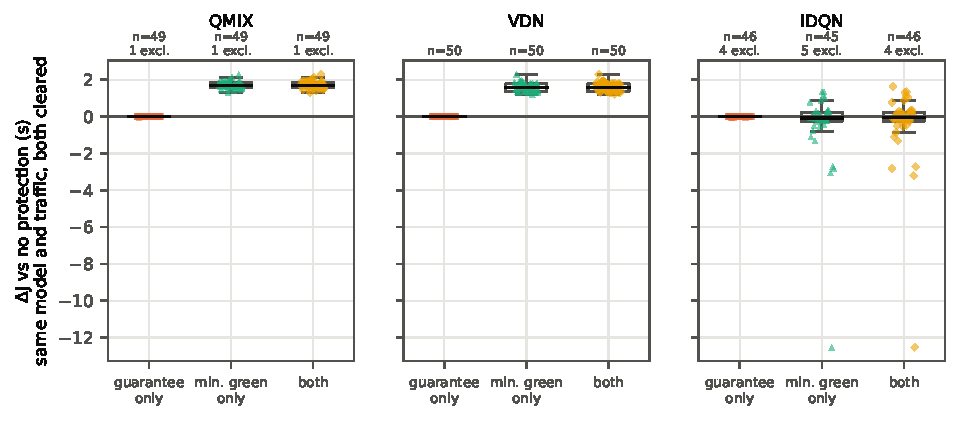
\includegraphics[width=\linewidth]{../figures/fig2a_paired_dJ}\\[2mm]
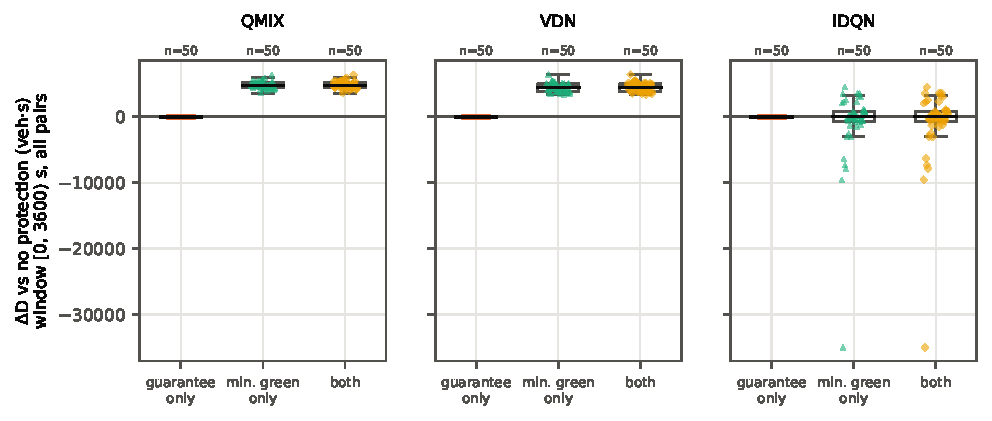
\includegraphics[width=\linewidth]{../figures/fig2b_paired_dD}
\caption{Paired effects of each protection relative to the same model and traffic without protection. Top:
$\Delta J$ (pairs where both runs clear; excluded pairs counted). Bottom: $\Delta D$ over the demand window
(all pairs).}
\label{fig:paired}
\end{figure}

\begin{figure}[t]
\centering
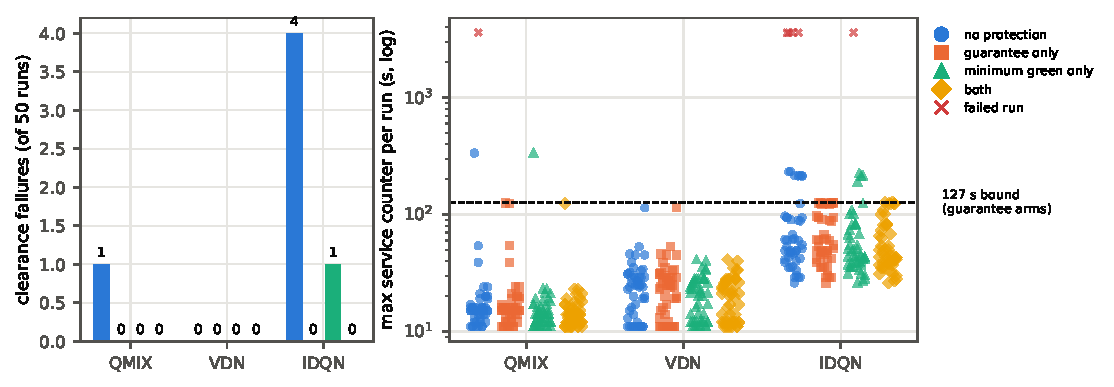
\includegraphics[width=\linewidth]{../figures/fig3_failures_and_service}
\caption{Left: clearance failures per method and arm. Right: maximum service counter per run (log scale);
the dashed line is the 127\,s bound that holds for the arms with the guarantee.}
\label{fig:service}
\end{figure}

\begin{figure}[t]
\centering
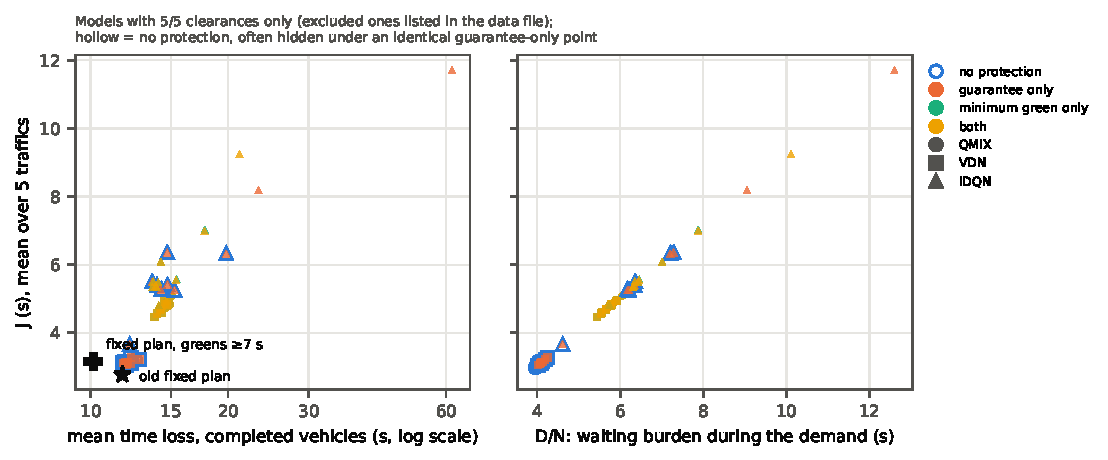
\includegraphics[width=\linewidth]{../figures/fig4_metric_tradeoff}
\caption{Indicator trade-offs: mean $J$ against mean time loss of completed vehicles (left) and against
$\bar D$ (right), for models that cleared all five traffics; excluded models are listed in the data file.}
\label{fig:tradeoff}
\end{figure}

\section{Discussion}
\paragraph{Failures are a property of the evaluation, not noise.} The failures are rare (6 of 300 runs
without the guarantee) but systematic in kind: a lone vehicle after the demand, facing a greedy policy whose
inputs barely change. Metrics computed on completed vehicles or on cleared runs do not register them; the
failed QMIX run has a mean time loss of 11.9\,s for its completed vehicles while one vehicle waits 3{,}600\,s.
Reporting the number of failures, keeping them out of averages, and using an indicator defined for every run
($D$) change what can be concluded.

\paragraph{The guarantee is cheap here because it is rarely needed.} On these traffics the guarantee repaired
every failure at no measurable cost, but only because it acted after the demand. Whether it is cheap when
secondary demand is light but persistent during a loaded period is untested; the prepared robustness study
targets exactly that.

\paragraph{The minimum green exposes a dependence on very short greens.} QMIX and VDN policies spend most of
their greens in the 2\,s minimum the executor allows. Imposing 7\,s at inference removes that behaviour and
costs 1.2--2.3\,s of waiting per vehicle. This measures the brittleness of these policies to a constraint they
were not trained with, not the value of the constraint itself, nor what a policy trained under it can achieve.
The single-seed pilots trained with the constraint are an exploratory, unfavourable signal on that question;
they do not predict whether a full campaign would close the gap to the re-optimised fixed plan or not.

\paragraph{Relation to the literature.} The comparison supports the concern that learned controllers are often
compared with weak references \cite{ault2020interpretable}: here, a fixed plan re-optimised under the same
constraint is not beaten by any cleared run of the historical policies constrained at evaluation (299 of 300
runs; the other failed to clear). Whether policies trained under the constraint would do better is not
established here. The lone-vehicle failure is a learned-controller counterpart of
the starvation that queue-based pressure control can produce for lightly loaded movements \cite{wu2018delay}.

\section{Limitations and scope}
\begin{itemize}
\item One corridor geometry and one demand level; five development traffics that had already been inspected.
\item The protections were added at evaluation time to policies trained without them; the effect of training
with them, and any effect of cooperation, are not measured here.
\item The constrained fixed plan was selected on the same design and validation samples as the original plan.
\item The comparison under the common constraint is asymmetric: a fixed plan re-optimised for the constraint
against learned policies constrained only at evaluation. Policies trained under the constraint exist only as
single-seed pilots.
\item The 127\,s bound applies to the service counter under the stated executor assumptions; it is not a bound
on a vehicle's total waiting or travel time.
\item Stop-line crossings are logged for the main axis only.
\end{itemize}

\section{Reproducibility}
Code, plans fixed before the runs, run ledgers with checkpoint and manifest hashes, derived data and figure
scripts are provided (Appendix~\ref{app:trace}). Software: Python 3.7.16, NumPy 1.21.6, PyTorch 1.13.1 (CPU),
SUMO 1.25.0, Windows.

\section*{Prepared but not executed}
A robustness validation on new traffics designed to stress service (persistent sparse secondary demand,
time-varying demand, isolated vehicles at the end of the demand), and a retraining campaign with the
protections, with new validation and final-test traffics, are specified with their analysis rules and costs.
The decision to run the retraining campaign will be taken after the robustness study and a full reading of the
closest works; \tocomplete{results}.

\appendix
\section{Technical traceability}\label{app:trace}
\begin{itemize}
\item Frozen learning and evaluation code: commit \texttt{8c14f32}; protected evaluator (masks, counters,
signal read-back): commit \texttt{3611383}, whose frozen part is identical to \texttt{8c14f32}.
\item Ablation plan fixed before the runs: fingerprint \texttt{c9a4c6d8\ldots} (600 cells; 550 new, 50 reused
with file hashes recorded and re-verified after the runs); analysis and indicator code committed before the
runs (study workspace commit \texttt{e0557af}).
\item Checkpoints: the 30 selected checkpoints verified by SHA-256 against the selection records before
copying; traffic manifests verified identical across the two earlier studies that used them.
\item Checks after the runs: 0 SUMO signal mismatches in 550 new runs; counters reconstructed from logs equal
to the logged counters in 100/100 runs; counter $\le$ 127\,s in every run with the guarantee; realised greens
$\ge$ 7\,s in every run with the minimum green.
\item Figures are produced by \texttt{figures/make\_figures.py}; the plotted values are in
\texttt{figures/data/}.
\item Tests: the 31 tests of the constrained fixed-plan search were run on the Windows stack above (terminal
output ``Ran 31 tests in 1548.888s'', ``OK'', exit status 0, transmitted by the operator; no log file of that
run is retained); the indicator and robustness tools have 11 unit tests run on the Windows stack (log retained)
and 10 tests of the robustness analysis on synthetic outputs.
\end{itemize}

\bibliographystyle{plainnat}
\bibliography{references}
\end{document}
